\documentclass[12pt]{article}   
\input packages
\input defs

\title{\bf Unified Engineering\\ 16.002 Signals and Systems\\ Review of Solving Ordinary Differential Equations}

\author{Jonathan P. How \\
	Massachusetts Institute of Technology \\ \texttt{jhow@mit.edu}
}

\date{}
\parskip = 12pt
\begin{document}
\jreset{1}
\maketitle

The goal is to discuss a simple solution methodology for ordinary differential equations -- these are assumed to be linear and the derivatives are only with respect to one variable.
So
$$
\dfrac{dy(t)}{dt} + y(t) = 3
$$
is an ODE, but
$$
\dfrac{dy(t)}{dt} + y^3(t) = 3
$$
isn't (it is nonlinear), and neither is (function of more than one variable)
$$
\dfrac{d^2y(x,w)}{dx^2} +\dfrac{d^2y(x,w)}{dw^2} = 3.
$$
Writing $\dot y(t) \equiv \dfrac{dy(t)}{dt}$, the basic form of an ODE is:
$$
y^{(n)}(t) + a_1 y^{(n-1)}(t)+\ldots+ a_{n-2}\ddot y(t) + a_{n-1} \dot y(t) + a_n y(t) = c w(t)
$$
where $w(t)$ is the input that is often constant, but can be a function of time, and the coefficients $a_i$ and $c$ are constant.

\section{Method of Assumed Solutions}
The solution approach is to \textbf{assume the form of an answer and then verify that it is the solution} (method of assumed solutions), which typically involves finding the unknown constants in the assumed form of the solution to ensure that the ODE is satisfied. This solution process must be executed in two steps. 
\begin{enumerate}
\item The \textbf{first} is to split the answer into two parts -- the homogeneous part $y_h(t)$ and the forced part $y_f(t)$, so that 
$$
y(t) = y_h(t) + y_f(t)
$$
where, by definition, the homogeneous part solves the equation
$$
y_h^{(n)}(t) + a_1 y_h^{(n-1)}(t)+\ldots+ a_{n-2}\ddot y_h(t) + a_{n-1} \dot y_h(t) + a_n y_h(t) = 0
$$
and we select $y_f(t)$ to satisfy
$$
y_f^{(n)}(t) + a_1 y_f^{(n-1)}(t)+\ldots+ a_{n-2}\ddot y_f(t) + a_{n-1} \dot y_f(t) + a_n y_f(t) = c w(t).
$$
%
Note that if we sum these two equations, 
\beas
&& y_h^{(n)}(t) + a_1 y_h^{(n-1)}(t)+\ldots+ a_{n-2}\ddot y_h(t) + a_{n-1} \dot y_h(t) + a_n y_h(t) \\ &+& \left(
y_f^{(n)}(t) + a_1 y_f^{(n-1)}(t)+\ldots+ a_{n-2}\ddot y_f(t) + a_{n-1} \dot y_f(t) + a_n y_f(t)\right) \\ &=& 
y^{(n)}(t) + a_1 y^{(n-1)}(t)+\ldots+ a_{n-2}\ddot y(t) + a_{n-1} \dot y(t) + a_n y(t)  
= c w(t)
\eeas
so that $y(t) = y_h(t) + y_f(t)$ is a solution to the original ODE.

\item The \textbf{second} step is to assume a particular form for $y_h(t)$ (usually an exponential)
$$
y_h(t) = Ce^{pt}
$$ 
where the constants $C$ and $p$ have to be found to ensure that the ODE is satisfied.
\end{enumerate}

\noindent
\textbf{Note:} that initial conditions specified for the problem must be applied to the complete $y(t)$.

\newpage
\section{First Order Systems}
Specializing to a first order ODE (one derivative) $$\dot y(t) + a y(t) = c w(t)$$ and substituting  $y_h(t)$ gives
$$
Cp e^{pt} + a Ce^{pt} = 0 
$$ 
where the right hand side is zero because this is the homogeneous solution. Note that the $Ce^{pt}$ terms can be canceled out, leaving $p+a=0$, so we must have that $p=-a$ to satisfy this ODE.
Thus we know that
$$
y_h(t) = Ce^{-at}.
$$ 
Had the input been constant $w(t) = B$, then we know that $y_f(t) = cB/a$ is a possible solution (all derivatives of this $y_f(t)$ are zero) and thus
$$
y(t) = y_h(t) + y_f(t) = \dfrac{cB}{a} + Ce^{-at}
$$
where the coefficient $C$ can now be found by ensuring that the initial condition is satisfied.

For example, if we had been told that $y(0)=0$, then $y(0)= \dfrac{cB}{a} + Ce^{-a0} = \dfrac{cB}{a} + C = 0$, which 
means that $C = -\dfrac{cB}{a}$ and
$$
y(t) = y_h(t) + y_f(t) = \dfrac{cB}{a} (1-e^{-at})
$$
This solution makes sense (and satisfies the ODE) because $y(0)=0$ and $\lim_{t \to \infty}y(t) = cB/a$, which is the forced solution.

\newpage
\subsection{Useful guess table for forced solutions}
For many common inputs, the method of assumed solutions starts by trying one of the forms below for the forced response $y_f(t)$:

\begin{center}
\begin{tabular}{|c|c|}
\hline
Input $w(t)$ & Try this form for $y_f(t)$ \\
\hline
Constant $B$ & $C$ \\
\hline
$e^{\beta t}$ & $C e^{\beta t}$ \\
\hline
$\cos(\omega t)$ or $\sin(\omega t)$ & $C_1 \cos(\omega t)+C_2 \sin(\omega t)$ \\
\hline
Polynomial in $t$ of degree $m$ & polynomial in $t$ of degree $m$ \\
\hline
\end{tabular}
\end{center}
If the input is a sum of terms, use a sum of corresponding trial forms for $y_f(t)$.

\subsubsection*{Resonance rule (repeated-root fix)}
If your trial $y_f(t)$ contains any term already present in $y_h(t)$, the trial is not linearly independent and will fail. In that case, multiply the trial by $t$ enough times to make it independent:
$$
y_f^{\rm new}(t) = t^r y_f^{\rm trial}(t)
$$
where $r$ is the multiplicity of the overlap with the homogeneous solution. For example, if $e^{-3t}$ already appears in $y_h(t)$, then try $t e^{-3t}$; if $t e^{-3t}$ also appears, then try $t^2 e^{-3t}$.

\begin{example} (first order, constant input) 
If $y(0)=4$, solve for $y(t)$ given 
$$\dot y(t) + 3 y(t) = 9 $$
Here we know that $y_h(t) = Ce^{pt}$ would yield
$$
Cpe^{pt} + 3 Ce^{pt} = 0 \quad \to \quad p=-3
$$
and $y_h(t) = Ce^{-3t}$. Further we can guess that $y_f(t) = 9/3=3$, yielding 
$$
y(t) = y_h(t) + y_f(t) = 3 + Ce^{-3t}
$$
To impose the initial condition, let $y(0)=3+C=4$, so $C=1$ and $y(t) = 3 + e^{-3t}$.
\end{example}

\begin{example} (first order, exp input) Consider the same system with different input $w(t) = e^{\beta t}$. We can try an assumed forced response of the form
$y_f(t) = C e^{\beta t}$ to get
$$
\dot y_f(t) + 3 y_f(t) =  e^{\beta t} \quad \to \quad C\beta e^{\beta t} + 3 C e^{\beta t} = e^{\beta t}
$$
which will true if $C(\beta + 3) = 1$ or $C=1/(\beta+3)$, which works provided that $\beta \neq -3$, because if it did, then this forced solution satisfies the homogeneous ODE and would give zero on the LHS resulting in a contradiction.  
Here the overall solution is
$$
y(t) = y_h(t) + y_f(t) = C e^{-3t} + \dfrac{e^{\beta t}}{3+\beta}
$$
where $y(0)=4$ would mean that $C + \dfrac{1}{3+\beta} = 4$ and 
$$y(t) = (4- \dfrac{1}{3+\beta}) e^{-3t}+ \dfrac{1}{3+\beta}e^{\beta t}$$
\end{example}

\begin{example} (first order, repeated roots) If the input was actually of the form $w(t) = e^{-3 t}$, then we would have to assume a different forced solution of the form $y_f(t) = C_2t e^{\beta t}$ yielding
$$
\dot y_f(t) + 3 y_f(t) =  e^{-3 t} \quad \to \quad -3 C_2t e^{-3 t} + C_2 e^{-3 t} + 3 C_2t e^{-3 t} = e^{-3 t}
$$
Since the first and last terms of the lefthand side cancel, we need $C_2=1$ to satisfy the equation. The combined solution would now be
$$
y(t) = y_h(t) + y_f(t) = C e^{-3t} + te^{-3t}
$$
where $y(0)=4$ would mean that $C=4$ and $y(t) = (4 + t)e^{-3t}$.
\end{example}

\begin{figure}[h]
\def\tm{3}
{\centering 
\begin{tikzpicture}[scale=1] 
\begin{axis} [width=\textwidth, height=2.5in, smooth, no markers, grid, domain=0:\tm, xmax=\tm, ymax=4, xmin=0, ymin=-0.5, xlabel={$t$},ylabel={Forced Response to $e^{\beta t}$}]
\pgfmathsetmacro{\b}{-0.1}
\addplot+[samples=200,color=red!90!blue,line width=1]{(4*\b+11)*exp(-3*x)/(\b+3) + exp(\b*x)/(\b+3)};
\addplot+[samples=200,color=blue!90!blue,line width=2]{(4+x)*exp(-3*x)};
\legend{$y(t)$ with $w(t) = e^{\b t}$,$y(t)$ with $w(t) = e^{-3 t}$,c,d,e}
%\node at (axis cs:1,.15) [anchor = north east] {Frequency is \b};
\end{axis}  
\end{tikzpicture}   }
\caption{Comparison of two first order system responses to different exponential inputs.}
\end{figure}

\subsection{Sinusoidal Inputs}
Consider the same first order system with a different input $w(t) = \cos(\omega t)$. 
We can try an assumed forced response of the form
$y_f(t) = C \cos(\omega t)$ but we might anticipate some issues since $\dot y$ will be $-C \omega \sin(\omega t)$ and so the functional forms don't cancel out nicely.

More generally this can be done for a complex input $w(t) = e^{i \omega t}$ and then we take the real or imaginary part of the solution depending on the type of input we want to consider ($\cos$ or $\sin$). Note that now we have to assume that 
$y_f(t) = C e^{i \omega t}$, i.e. that the output is some scaled version of the input (seems reasonable as the system is linear).
$$
y_f(t) = C e^{i \omega t}, \quad \dot y_f(t) = i\omega C e^{i \omega t}
$$
so we have that 
$$
\dot y_f(t) + 3 y_f(t) =  e^{i \omega t} \quad \to \quad i\omega C e^{i \omega t} + 3 C e^{i \omega t} = e^{i \omega t}
$$
requiring that $C (3 + i\omega) = 1$ or $C=\dfrac{1}{(3 + i \omega)} = \dfrac{1}{\sqrt{9 + \omega^2}}e^{i\phi}$ where to find $\phi$ note that
$C=\dfrac{1}{(3 + i \omega)} = \dfrac{3 - i \omega}{9 + \omega^2}$, so $\tan(\phi) = \dfrac{-\omega}{3}$.

\begin{example} (first order, sinusoidal input) If the input happened to be $w(t) = \cos(3t)$ so that $\omega = 3$, the forced output would be the real part of the signal computed above $y_f(t)={\tt real}\left(\dfrac{1}{\sqrt{9+9}}e^{i\phi}\right)$ with $\phi = \arctan\left(\dfrac{-3}{3}\right) = -\dfrac{\pi}{4}$, so that
$$
y_f(t) = \dfrac{1}{\sqrt{18}} \cos\left(3t -\dfrac{\pi}{4}\right)
$$
the total solution would be 
$$
y(t) = y_h(t) + y_f(t) = C e^{-3t} + \dfrac{1}{\sqrt{18}} \cos\left(3t -\dfrac{\pi}{4}\right)
$$
and $y(0)=4$ implies that $C + \dfrac{1}{\sqrt{18}}\dfrac{1}{\sqrt{2}} = C + \dfrac{1}{\sqrt{36}}=4$ or $C=4-\dfrac{1}{6}$. Substituting gives
$$
y(t) = \dfrac{23}{6} e^{-3t} + \dfrac{\sqrt{2}}{6} \cos\left(3t -\dfrac{\pi}{4}\right)
$$
\end{example}

\begin{figure}[h]
\def\tm{6}
{\centering 
\begin{tikzpicture}[scale=1] 
\begin{axis} [width=\textwidth, height=2.5in, smooth, no markers, grid, domain=0:\tm, xmax=\tm, ymax=4, xmin=0, ymin=-0.5, xlabel={$t$},ylabel={Forced Response to cos(3t)}]
\pgfmathsetmacro{\w}{3}
\pgfmathsetmacro{\p}{atan(-\w/3)}
\addplot+[samples=200,color=red!90!blue,line width=2]{23*exp(-3*x)/6 + sqrt(2) * cos(deg(\w*x )+ \p)/6};
\addplot+[samples=200,color=green!50!blue,line width=2,dashed]{sqrt(2) * cos(deg(\w*x) +\p)/6};
\legend{$y(t)$ with $w(t) = \cos{3t}$,$w(t)/6$ - phase shift \p,c,d,e}
%\node at (axis cs:1,.15) [anchor = north east] {Frequency is \b};
\end{axis}  
\end{tikzpicture}   }
\caption{First order response to sinusoidal input showing rapid initial decay to a shifted sinusoid. Shifted input provided as a reference.}
\end{figure}

\section{Higher Order Systems}
For higher order systems, the method of assumed solutions gets a bit more complicated as we end up with higher order equations to solve for $p$. This is tractable for second order ODE (solve a quadratic), but requires a computer for higher order. 

If the roots of the quadratic are real $p_1$ and $p_2$, but not repeating, then the homogeneous solution will be of the form
\begin{eqnarray}
y_h(t) &=& C_1 e^{p_1t} + C_2 e^{p_2t} 
\end{eqnarray}
which is combined with the forced solution to obtain the final result. Had the poles been repeated, then we would have to consider homogeneous solutions of the form 
\begin{eqnarray}
y_h(t) &=& (C_1 + C_2t) e^{pt} 
\end{eqnarray}
giving
\begin{eqnarray}
\dot y_h(t) &=& C_2 e^{pt} + p(C_1 + C_2t) e^{pt},\\ \ddot y_h(t) &=& pC_2 e^{pt} + p(C_2) e^{pt} + p^2(C_1 + C_2t) e^{pt}
\end{eqnarray}

\begin{example}
(real, non-repeating poles; constant input) solve $$\ddot y(t) + 3 \dot y(t) + 2 y(t) = 1$$ for positive $t$ given initial conditions (IC) that $y(0)=1$ and $\dot y(0) = 0$. Here assuming that $y_h(t)=Ce^{pt}$, substitution gives
$$
p^2Ce^{pt} +3 pCe^{pt} + 2Ce^{pt} = 0
$$
requiring that $p^2+3p+2=0$ with roots $p=-1,-2$ so
\begin{eqnarray}
y_h(t) &=& C_1 e^{-t} + C_2 e^{-2t} 
\end{eqnarray}
The forced solution for a constant input is guessed to be $y_f(t) = 1/2$, so 
\begin{eqnarray}
y(t) &=& 0.5 + C_1 e^{-t} + C_2 e^{-2t} 
\end{eqnarray}
Impose the IC to get $y(0)=1 = 0.5 + C_1+C_2$ and $\dot y(0)= 0 = -C_1-2C_2$. So $C_1=-2C_2$ and $-C_2=0.5$, $C_1=1$. The final result is that
$$
y(t) = 0.5 +e^{-t} -0.5 e^{-2t}
$$
\end{example}

\begin{example}
(real, repeating poles; constant input) solve $$\ddot y(t) + 2 \dot y(t) + 1 y(t) = 1$$ (repeated root at $p=-1$) 
for positive $t$ given initial conditions (IC) that $y(0)=1$ and $\dot y(0) = 1$. 
Here assuming that $y_h(t) = (C_1 + C_2t) e^{pt}$, with $p=-1$ substitution gives
$$
-2C_2e^{-t} + (C_1 + C_2t) e^{-t} + 2(C_2 e^{-t} -(C_1 + C_2t) e^{-t}) + (C_1 + C_2t) e^{-t} = 0
$$
divide through
$$
-2 C_2  + (C_1 + C_2t) + 2(C_2 -(C_1 + C_2t)) + (C_1 + C_2t)  = 0
$$
giving
$$
C_1(-2+1+1) + C_2(-2 + t +2 -2t +t) = 0
$$
so the solution does satisfy the ODE. The initial conditions can then be used to determine $C_1$ and $C_2$ using the total solution
\begin{eqnarray}
y(t) &=& 1 + (C_1 + C_2t) e^{-t} 
\end{eqnarray}
Impose the IC to get $y(0)=1 = 1 + C_1$ so $C_1=0$ and $\dot y(0)= 1 = C_2 $. 
The final result is that
$$
y(t) = 1 + te^{-t} 
$$
\end{example}

\begin{example} (real, non-repeating poles; exp input) 
Solve $$\ddot y(t) + 3 \dot y(t) + 2 y(t) = e^{\beta t}$$ 
for positive $t$ given initial conditions (IC) that $y(0)=1$ and $\dot y(0) = 0$. The homogeneous solution is as above, but the forced solution is now $y_f(t)= C e^{\beta t}$ where we assume that $\beta \neq -1,-2$. Substitute to get
$$
C \beta^2 e^{\beta t} +3 \beta Ce^{\beta t} + 2Ce^{\beta t} = e^{\beta t}
$$
which requires that $C=\dfrac{1}{\beta^2 + 3 \beta + 2 }$.
The full solution is then
\begin{eqnarray}
y(t) &=& C_1 e^{-t} + C_2 e^{-2t} + \dfrac{e^{\beta t}}{\beta^2 + 3 \beta + 2 }
\end{eqnarray}
Impose the IC to get $y(0)=1 = C_1+C_2 + \dfrac{1}{\beta^2 + 3 \beta + 2 }$ 
and $\dot y(0)= 0 = -C_1-2C_2 + \dfrac{\beta}{\beta^2 + 3 \beta + 2 }$. 
So $C_1=-2C_2 + \dfrac{\beta}{\beta^2 + 3 \beta + 2 }$ and
$$
\dfrac{\beta^2 + 3\beta +1}{\beta^2 + 3 \beta + 2 } = -C_2 + \dfrac{\beta}{\beta^2 + 3 \beta + 2 }
$$
so
$$
C_2 = -\dfrac{\beta^2 + 2\beta +1}{\beta^2 + 3 \beta + 2 }, \quad C_1 = 2 \dfrac{\beta^2 + 2\beta +1}{\beta^2 + 3 \beta + 2 } + \dfrac{\beta}{\beta^2 + 3 \beta + 2 } = \dfrac{2\beta^2 +5\beta +2}{\beta^2 + 3 \beta + 2 }
$$
The final result is that
$$
y(t) =  \dfrac{(2\beta^2 + 5 \beta +2)e^{-t}  -    (\beta^2 + 2\beta +1)e^{-2t}  + e^{\beta t}}{(\beta + 1)(\beta + 2)}
$$
which simplifies a bit because $2\beta^2 + 5 \beta +2 = (2\beta + 1)(\beta + 2)$ and  $\beta^2 + 2\beta + 1 = (\beta + 1)(\beta + 1)$
$$
y(t) =  \dfrac{(2\beta +1)e^{-t}}{(\beta + 1)}
-\dfrac{(\beta +1)e^{-2t}  }{\beta + 2}
+ \dfrac{e^{\beta t}}{(\beta + 1)(\beta + 2)}
$$
\end{example}

\subsection{Complex Roots} Further, for second order, one can end up with complex solutions for $p$, implying that sinusoids are involved since we know that $$e^{i\theta} = \cos \theta + i \sin \theta$$ meaning that
$$
\cos \theta = \dfrac{e^{i \theta} + e^{-i \theta}}{2} \quad {\rm and} \quad
\sin \theta = \dfrac{e^{i \theta} - e^{-i \theta}}{2i}
$$ 
Thus if we substitute the assumed solution into a second order ODE and solve for $p$ to a obtain a complex solution pair $p=p_r\pm i p_i$ (this will not always be the case), then
\begin{eqnarray}
y_h(t) &=& C_1 e^{(p_r + i p_i)t} + C_2 e^{(p_r - i p_i)t} = e^{p_r t} ( C_1 e^{i p_i t} + C_2 e^{- i p_i t}) \\ 
&=&  e^{p_r t}\left[ \left(C_1+C_2\right) \dfrac{(e^{i p_i t} + e^{- i p_i t})}{2}  +i\left(C_1-C_2\right) \dfrac{(e^{i p_i t} - e^{- i p_i t})}{2i}\right] \\
&=&  e^{p_r t}\left[ \left(C_1+C_2\right) \cos(p_i t) +  i\left(C_1-C_2\right) \sin(p_i t) \right]
\end{eqnarray}
This second last step looks a bit ugly, but typically $C_2=C_1^*$ (they are complex conjugates of each other), and then $C_1+C_2 = 2{\tt real}(C_1)$ and $i(C_1-C_2) = -2{\tt imag}(C_1)$, so things simplify a bit.

\begin{example} (complex roots, constant input) solve $$\ddot y(t) + 2 \dot y(t) + 10 y(t) = 1$$ for positive $t$ given initial conditions (IC) that $y(0)=1$ and $\dot y(0) = 0$. 
Start with the homogeneous part: $ y_h(t) = C e^{pt}$ - substitute and cancel to get 
$$
p^2+2p+10 = 0
$$
with roots $p=-1\pm3i$ so that 
$$
y_h(t) = C_1 e^{(-1 + 3i )t} + C_2 e^{(-1 - 3i)t} 
$$
Now look at the forced part: Since the input is a constant, we can guess that the forced response will also be a constant (all derivatives are zero), so that $10y_f(t) = 1$, or $y_f(t)=0.1$.
Thus we have 
$$
y(t) = 0.1 + C_1 e^{(-1 + 3i )t} + C_2 e^{(-1 - 3i)t}
$$
Now we need to impose the IC:
\begin{eqnarray}
y(0) &=& 0.1 + C_1 e^{0} + C_2 e^{0} = 1 \quad \to C_1+C_2 = 0.9\\
\dot y(0) &=& C_1 (-1+3i) e^{0} + C_2 (-1-3i) e^{0} = 0 \quad \to C_1 = C_2\dfrac{(1+3i)}{-1+3i}
\end{eqnarray}
giving 2 equations in 2 unknowns. Solving gives
$$
C_2 (1 + \dfrac{1+3i}{-1+3i}) =  C_2 (\dfrac{6i}{-1+3i}) = 0.9
$$
so $C_2 = 0.9 \dfrac{-1+3i}{6i} = \dfrac{0.9(3+i)}{6}$ and $C_1 = \dfrac{0.9(3-i)}{6}$. Since in the case $p_r=-1$ and $p_i=3$, we get the simpler version of the response as 
\begin{eqnarray}
y(t) &=& 0.1 + C_1 e^{(-1 + 3i )t} + C_2 e^{(-1 - 3i)t}\\
&=&  0.1 + \frac{0.9(3-i)}{6} e^{(-1 + 3i )t} + \frac{0.9(3+i)}{6} e^{(-1 - 3i)t}\\
&=& 0.1 + e^{-t}(0.9\cos(3t) + \dfrac{1.8}{6}\sin(3t)) \label{8}
\end{eqnarray}
Confirming that $y(0)=0.1+0.9=1$ and 
$$\dot y(t) = -e^{-t}(0.9\cos(3t) + \dfrac{1.8}{6}\sin(3t)) + e^{-t}(-3\cdot0.9\sin(3t) + 3\dfrac{1.8}{6}\cos(3t))$$
so $\dot y(0) = -0.9 + 1.8/2 = 0$ as required.
We can simplify further by noting that 
\begin{equation}
y(t) = 0.1 + 0.9e^{-t}(\cos(3t) + \dfrac{1}{3}\sin(3t)) = 0.1 + 0.9\sqrt{1+(1/3)^2}e^{-t}\cos(3t + \phi) \label{9}
\end{equation}
where $\tan \phi = -1/3$.

\begin{figure}
{\centering 
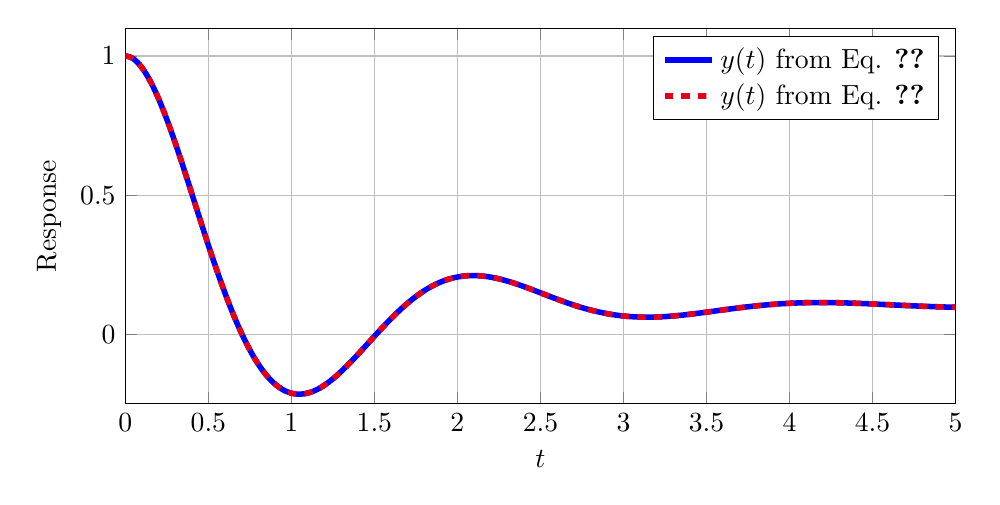
\begin{tikzpicture} 
\begin{axis} [width=\textwidth, height=2.5in, smooth, no markers, grid, domain=0:2, xmax=5, ymax=1.1, xmin=0, ymin=-0.25, xlabel={$t$},ylabel={Response}]
\pgfmathsetmacro{\p}{atan(-1/3)}
\addplot+[samples=200,color=blue,domain=0:5,line width=2]{0.1 + 0.9* exp(-x)*( cos(deg(3*x)) + sin(deg(3*x))/3 )};
\addplot+[samples=200,color=red!90!blue,dashed,domain=0:5,line width=2]{0.1 + 0.9* sqrt(1+(1/3)^2)*exp(-x)*cos(deg(3*x ) + \p) };
\legend{$y(t)$ from Eq. \ref{8},$y(t)$ from Eq. \ref{9},c,d,e}
\end{axis}  
\end{tikzpicture}} \vspace*{-0.25in}
\caption{Response of second order system with complex roots. Compares two equivalent representations of the same solution.}
\end{figure}
\end{example}

\begin{example} (complex roots, sinusoidal input) Note that other forced inputs can also be considered, such as a sinusoid, so that $w(t) = \cos(\omega t)$. For this example, 
$$\ddot y(t) + 2 \dot y(t) + 10 y(t) = \cos(\omega t)$$
More generally this can be done for a complex input $w(t) = e^{i \omega t}$ and then we take the real or imaginary part of the solution depending on the type of input we want to consider ($\cos$ or $\sin$). Note that now we have to assume that 
$y_f(t) = C e^{i \omega t}$, i.e. that the output is some scaled version of the input (seems reasonable as the system is linear).
$$
y_f(t) = C e^{i \omega t}, \quad \dot y_f(t) = i\omega C e^{i \omega t}, \quad \ddot y_f(t) = -\omega^2 C e^{i \omega t}
$$
so we have that 
$$
 -\omega^2 C e^{i \omega t} + 2i\omega C e^{i \omega t} + 10C e^{i \omega t} = e^{i \omega t}
$$
which can only be true if 
$$
C (10 - \omega^2 + 2\omega i) = 1 \quad \to \quad C = \dfrac{1}{10 - \omega^2 + 2\omega i} = \dfrac{10 - \omega^2 - 2\omega i}{(10 - \omega^2)^2 + 4\omega^2} = C_r + i C_i
$$
so the coefficient is complex.  Thus the forced response is
\begin{eqnarray}
y_f(t) &=& C e^{i \omega t} = (C_r+iC_i) (\cos(\omega t) + i\sin(\omega t))  \\
&=& (C_r \cos(\omega t) - C_i\sin(\omega t)) + i(C_r \sin(\omega t) + C_i \cos(\omega t)) 
\end{eqnarray}
where both $C_r = (10 - \omega^2)/((10 - \omega^2)^2 + 4\omega^2)$ and $C_i = -2\omega/((10 - \omega^2)^2 + 4\omega^2)$ depend on the input frequency $\omega$.
So if the input was $w(t) = (\cos \omega t )$, then we just take the real part of the forced output
\begin{eqnarray}
y_f(t) &=& \dfrac{(10 - \omega^2)}{((10 - \omega^2)^2 + 4\omega^2)} \cos(\omega t) + \dfrac{2\omega}{((10 - \omega^2)^2 + 4\omega^2)} \sin(\omega t)  \label{12}\\
&=& \dfrac{(10 - \omega^2)\cos(\omega t) +2\omega \sin(\omega t)}{((10 - \omega^2)^2 + 4\omega^2)} \\
&=& \dfrac{\cos(\omega t + \phi)}{\sqrt{(10 - \omega^2)^2 + 4\omega^2}} \label{14}
\end{eqnarray}
where $\tan \phi = -\dfrac{2\omega}{(10 - \omega^2)}$.

\begin{figure}[h]
{\centering 
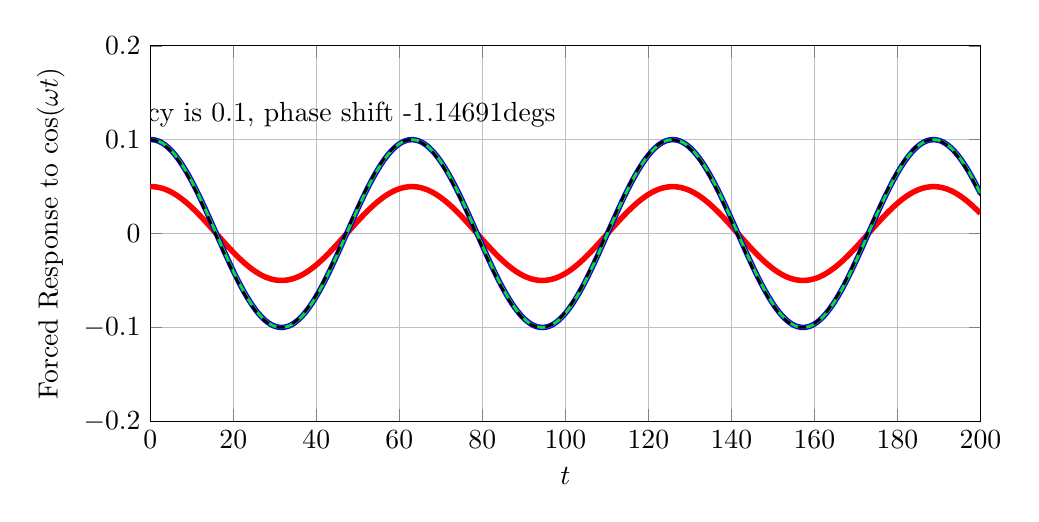
\begin{tikzpicture}[scale=1] 
\begin{axis} [width=\textwidth, height=2.5in, smooth, no markers, grid, domain=0:200, xmax=200, ymax=.2, xmin=0, ymin=-0.2, xlabel={$t$},ylabel={Forced Response to cos($\omega t$)}]
\pgfmathsetmacro{\w}{0.1}
\pgfmathsetmacro{\p}{atan2(-2*\w,10-\w^2)}
\addplot+[samples=200,color=red,line width=2]{ cos(deg(\w*x ) + \p)/20};
\addplot+[samples=200,color=red!10!blue,line width=2]{((10-\w^2)*cos(deg(\w*x )) + (2*\w)*sin(deg(\w*x )))/ ((10-\w^2)^2+4*\w^2))};
\addplot+[samples=200,color=green!90!blue,line width=1]{cos(deg(\w*x ) + \p) / sqrt((10-\w^2)^2+4*\w^2)};
\addplot+[samples=200,color=black,line width=1,dashed]{cos(deg(\w*x))/10};
%\legend{Freq is \w,phase shift \p,c,d,e}
\node at (axis cs:100,.15) [anchor = north east] {Frequency is \w, phase shift \trim \p degs};
\end{axis}  
\end{tikzpicture}}
{\centering 
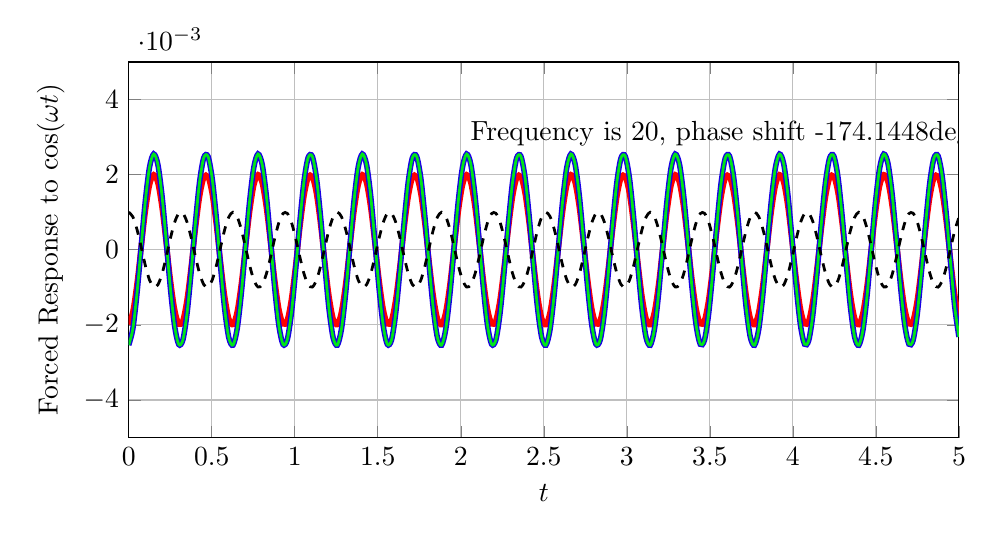
\begin{tikzpicture}[scale=1] 
\begin{axis} [width=\textwidth, height=2.5in, smooth, no markers, grid, domain=0:5, xmax=5, ymax=.005, xmin=0, ymin=-0.005, xlabel={$t$},ylabel={Forced Response to cos($\omega t$)}]
\pgfmathsetmacro{\w}{20}
\pgfmathsetmacro{\p}{atan2(-2*\w,10-\w^2)}
\addplot+[samples=200,color=red,line width=2]{ cos(deg(\w*x ) + \p)/500};
\addplot+[samples=200,color=red!10!blue,line width=2]{((10-\w^2)*cos(deg(\w*x )) + (2*\w)*sin(deg(\w*x )))/ ((10-\w^2)^2+4*\w^2))};
\addplot+[samples=200,color=green!90!blue,line width=1]{cos(deg(\w*x ) + \p) / sqrt((10-\w^2)^2+4*\w^2)};
\addplot+[samples=200,color=black,line width=1,dashed]{cos(deg(\w*x))/1000};
\node at (axis cs:2,.0025) [anchor = south west] {Frequency is \w, phase shift \trim \p degs};
\end{axis}  
\end{tikzpicture}}\vspace*{-0.1in}
\caption{Comparison of 2 forms of the forced response (only) (Equations \ref{12} and \ref{14}) for different frequency inputs. response in blue -- the input is in black, and the shifted (and scaled) input shown in red to show that the phase prediction (not amplitude) is accurate.}
\end{figure}
\end{example}

As before,  the total response is 
$$
y(t) = y_h(t) + y_f(t) = C_1 e^{(-1 + 3i )t} + C_2 e^{(-1 - 3i)t}  +
\dfrac{(10 - \omega^2)\cos(\omega t) +2\omega \sin(\omega t)}{\omega^4 -16\omega^2 +100}
$$
so $y(0)=1$ means that
$$
1 = C_1 + C_2 + \dfrac{(10 - \omega^2)}{\omega^4 -16\omega^2 +100}
$$
or
$$
C_1 + C_2 =  \dfrac{\omega^4 - 15\omega^2 + 90}{\omega^4 -16\omega^2 +100}
$$
Also
$$
\dot y(0) = C_1 (-1 + 3i ) + C_2 (-1 - 3i)  +
\dfrac{2\omega^2 }{\omega^4 -16\omega^2 +100} = 0
$$

This solves to give
$$
C_1 = \dfrac{3(\omega^4 -15\omega^2 +90) -j(\omega^4 -17\omega^2 +90)}{6(\omega^4 -16\omega^2 +100)}
$$
and $C_2=C_1^*$. Using the expressions in (3) to clean up the homogeneous part we get
\beas
y(t) &=& e^{-t}\left( 
\dfrac{3(\omega^4 -15\omega^2 +90)\cos(3t)+(\omega^4 -17\omega^2 +90)\sin(3t)}
{3(\omega^4 -16\omega^2 +100)} 
\right) \\ && +
\dfrac{(10 - \omega^2)\cos(\omega t) +2\omega \sin(\omega t)}{\omega^4 -16\omega^2 +100}
\eeas

\begin{figure}[t]
{\centering 
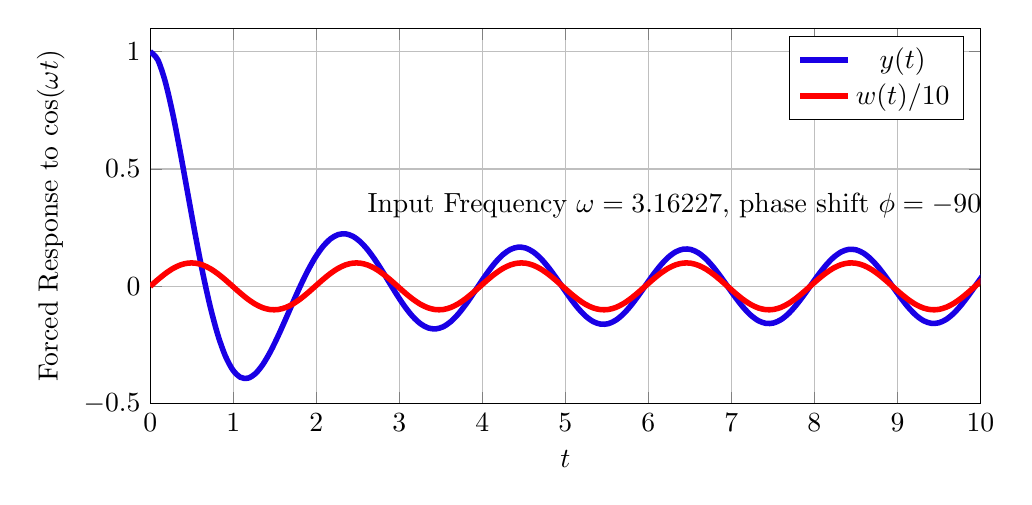
\begin{tikzpicture}[scale=1] 
\begin{axis} [width=\textwidth, height=2.5in, smooth, no markers, grid, domain=0:18, xmax=10, ymax=1.1, xmin=0, ymin=-0.5, xlabel={$t$},ylabel={Forced Response to cos($\omega t$)}]
\pgfmathsetmacro{\w}{sqrt(10)}
\pgfmathsetmacro{\p}{atan2(-2*\w,10-\w^2)}
\addplot+[samples=200,color=red!10!blue,line width=2]{exp(-x)*(3*(\w^4-15*\w^2+90)*cos(deg(3*x )) + (\w^4-17*\w^2+90)*sin(deg(3*x ))  )/ (\w^4-16*\w^2+100)/3)
+ ((10-\w^2)*cos(deg(\w*x )) + (2*\w)*sin(deg(\w*x )))/ (\w^4-16*\w^2+100)};
\addplot+[samples=200,color=red,line width=2]{ cos(deg(\w*x ) + \p)/10};
\legend{$y(t)$,$w(t)/10$,e}
\node at (axis cs:2.5,.25) [anchor = south west] {Input Frequency $\omega=\trim \w$, phase shift $\phi=\trim \p$ degs};
\end{axis}  
\end{tikzpicture}   } \vspace*{-0.25in}
\caption{Total response to sinusoidal input. Red line shows phase shifted (and scaled) input for comparison.}
\end{figure}

\newpage
\section{Solving ODEs in Python}
There are different solution approaches that one can use in Python to solve ODEs.

\noindent
\textbf{Shared utilities:} Common helper functions are defined here.
\bc
\begin{center}
\textbf{\texttt{scripts/ode\_common.py}}
\lstinputlisting{scripts/ode_common.py}
\end{center}
\ec

\noindent
\textbf{Symbolic:} The plotted symbolic/analytic cases are generated by these standalone scripts.
\bc
\begin{center} \tiny
\textbf{\texttt{scripts/01\_first\_order.py}}
\lstinputlisting{scripts/01_first_order.py}
\vspace{0.2in}
\textbf{\texttt{scripts/02\_second\_order\_real.py}}
\lstinputlisting{scripts/02_second_order_real.py}
\vspace{0.2in}
\textbf{\texttt{scripts/03\_second\_order\_complex.py}}
\lstinputlisting{scripts/03_second_order_complex.py}
\vspace{0.2in}
\textbf{\texttt{scripts/04\_second\_order\_repeated.py}}
\lstinputlisting{scripts/04_second_order_repeated.py}
\end{center}
\ec
\bc
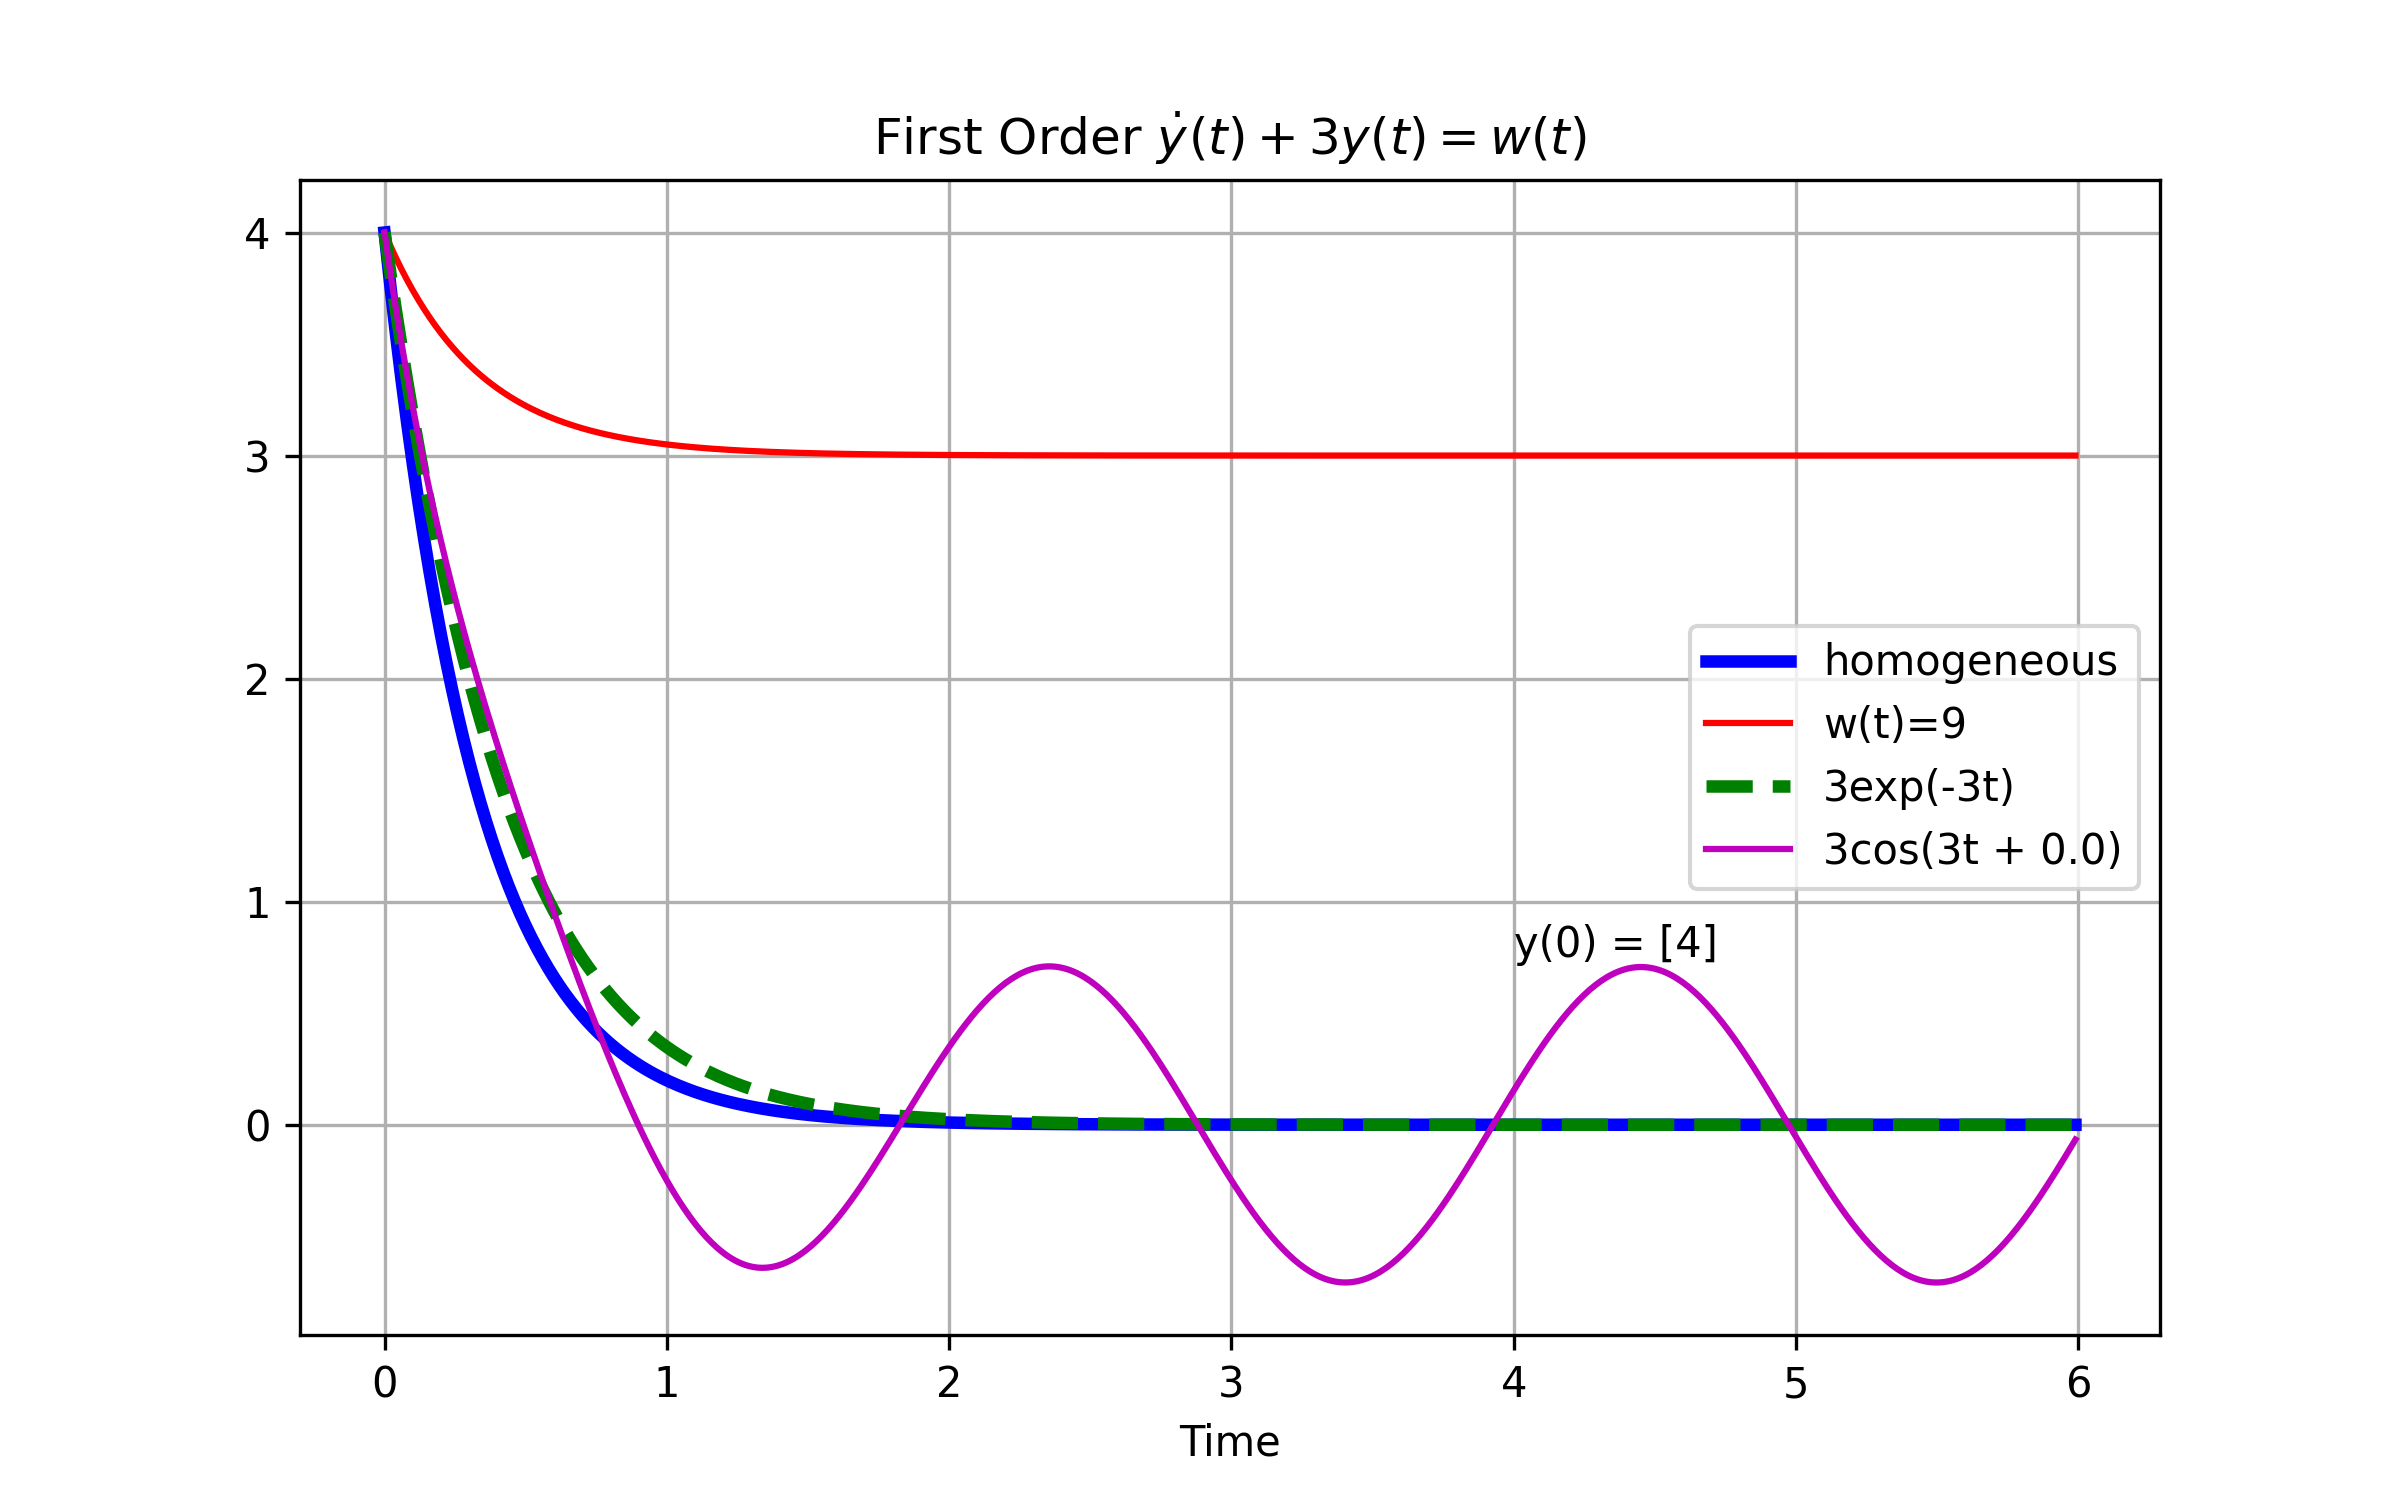
\includegraphics[width=6in]{figs/first_order.png}
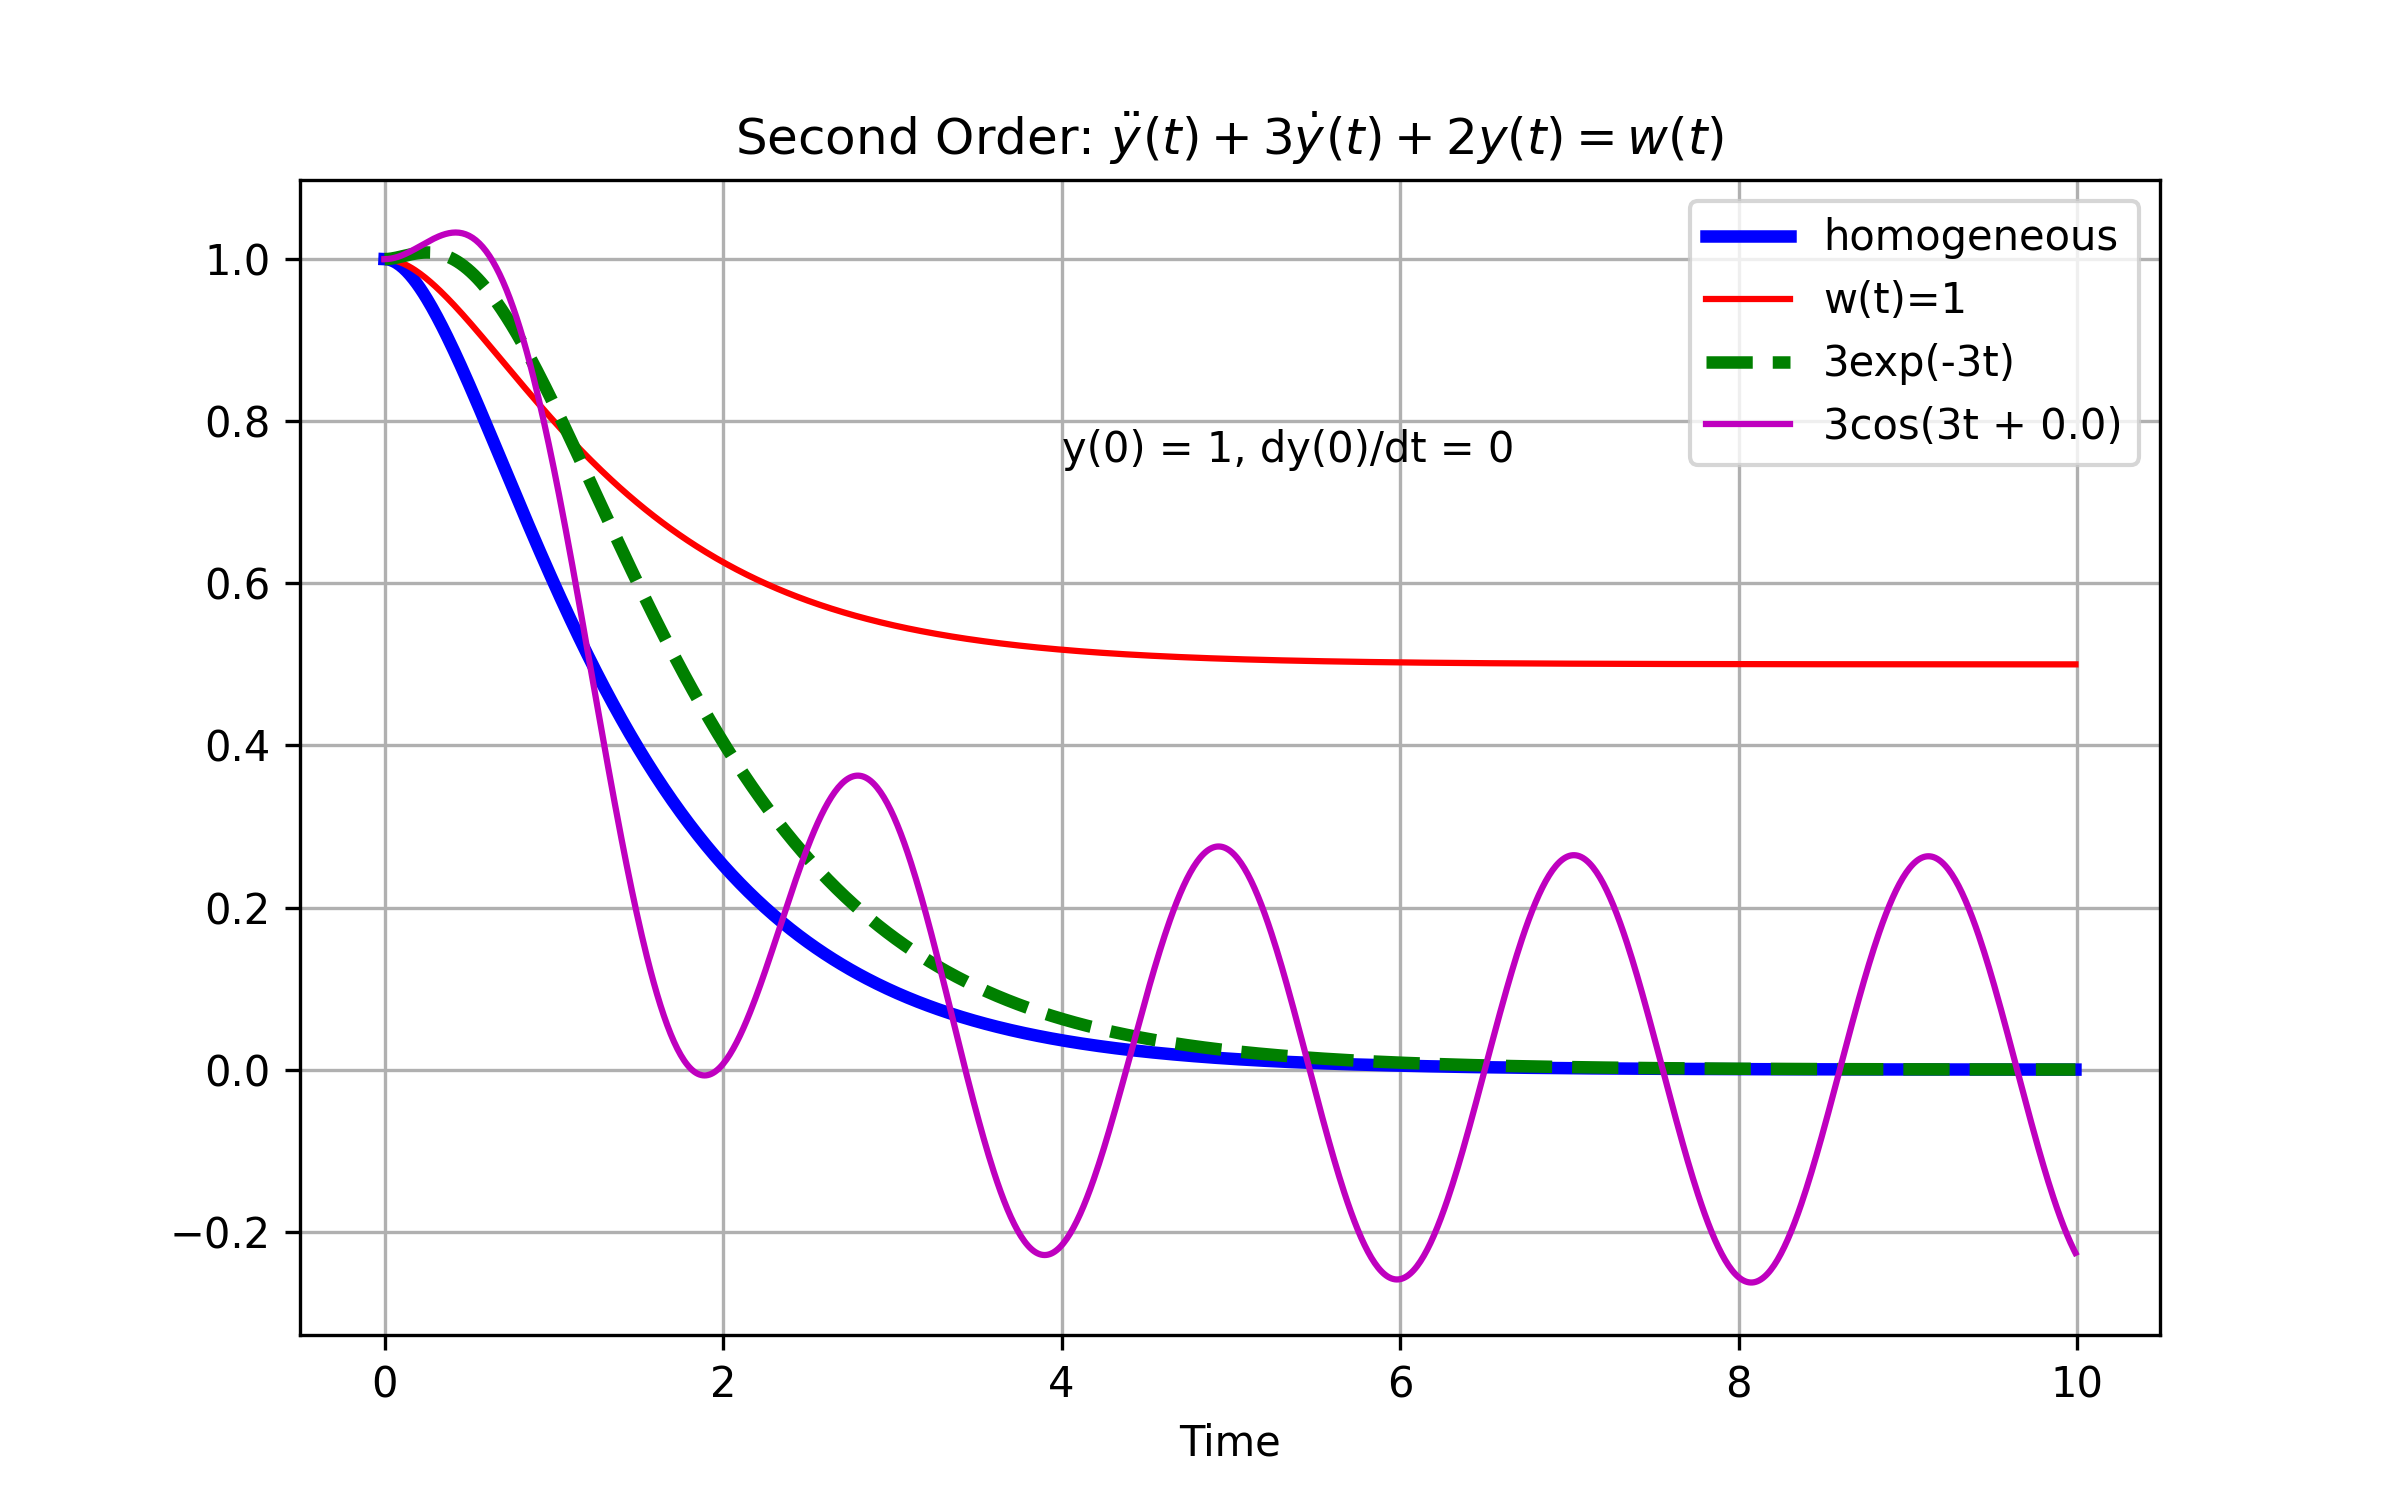
\includegraphics[width=6in]{figs/second_order.png} \\
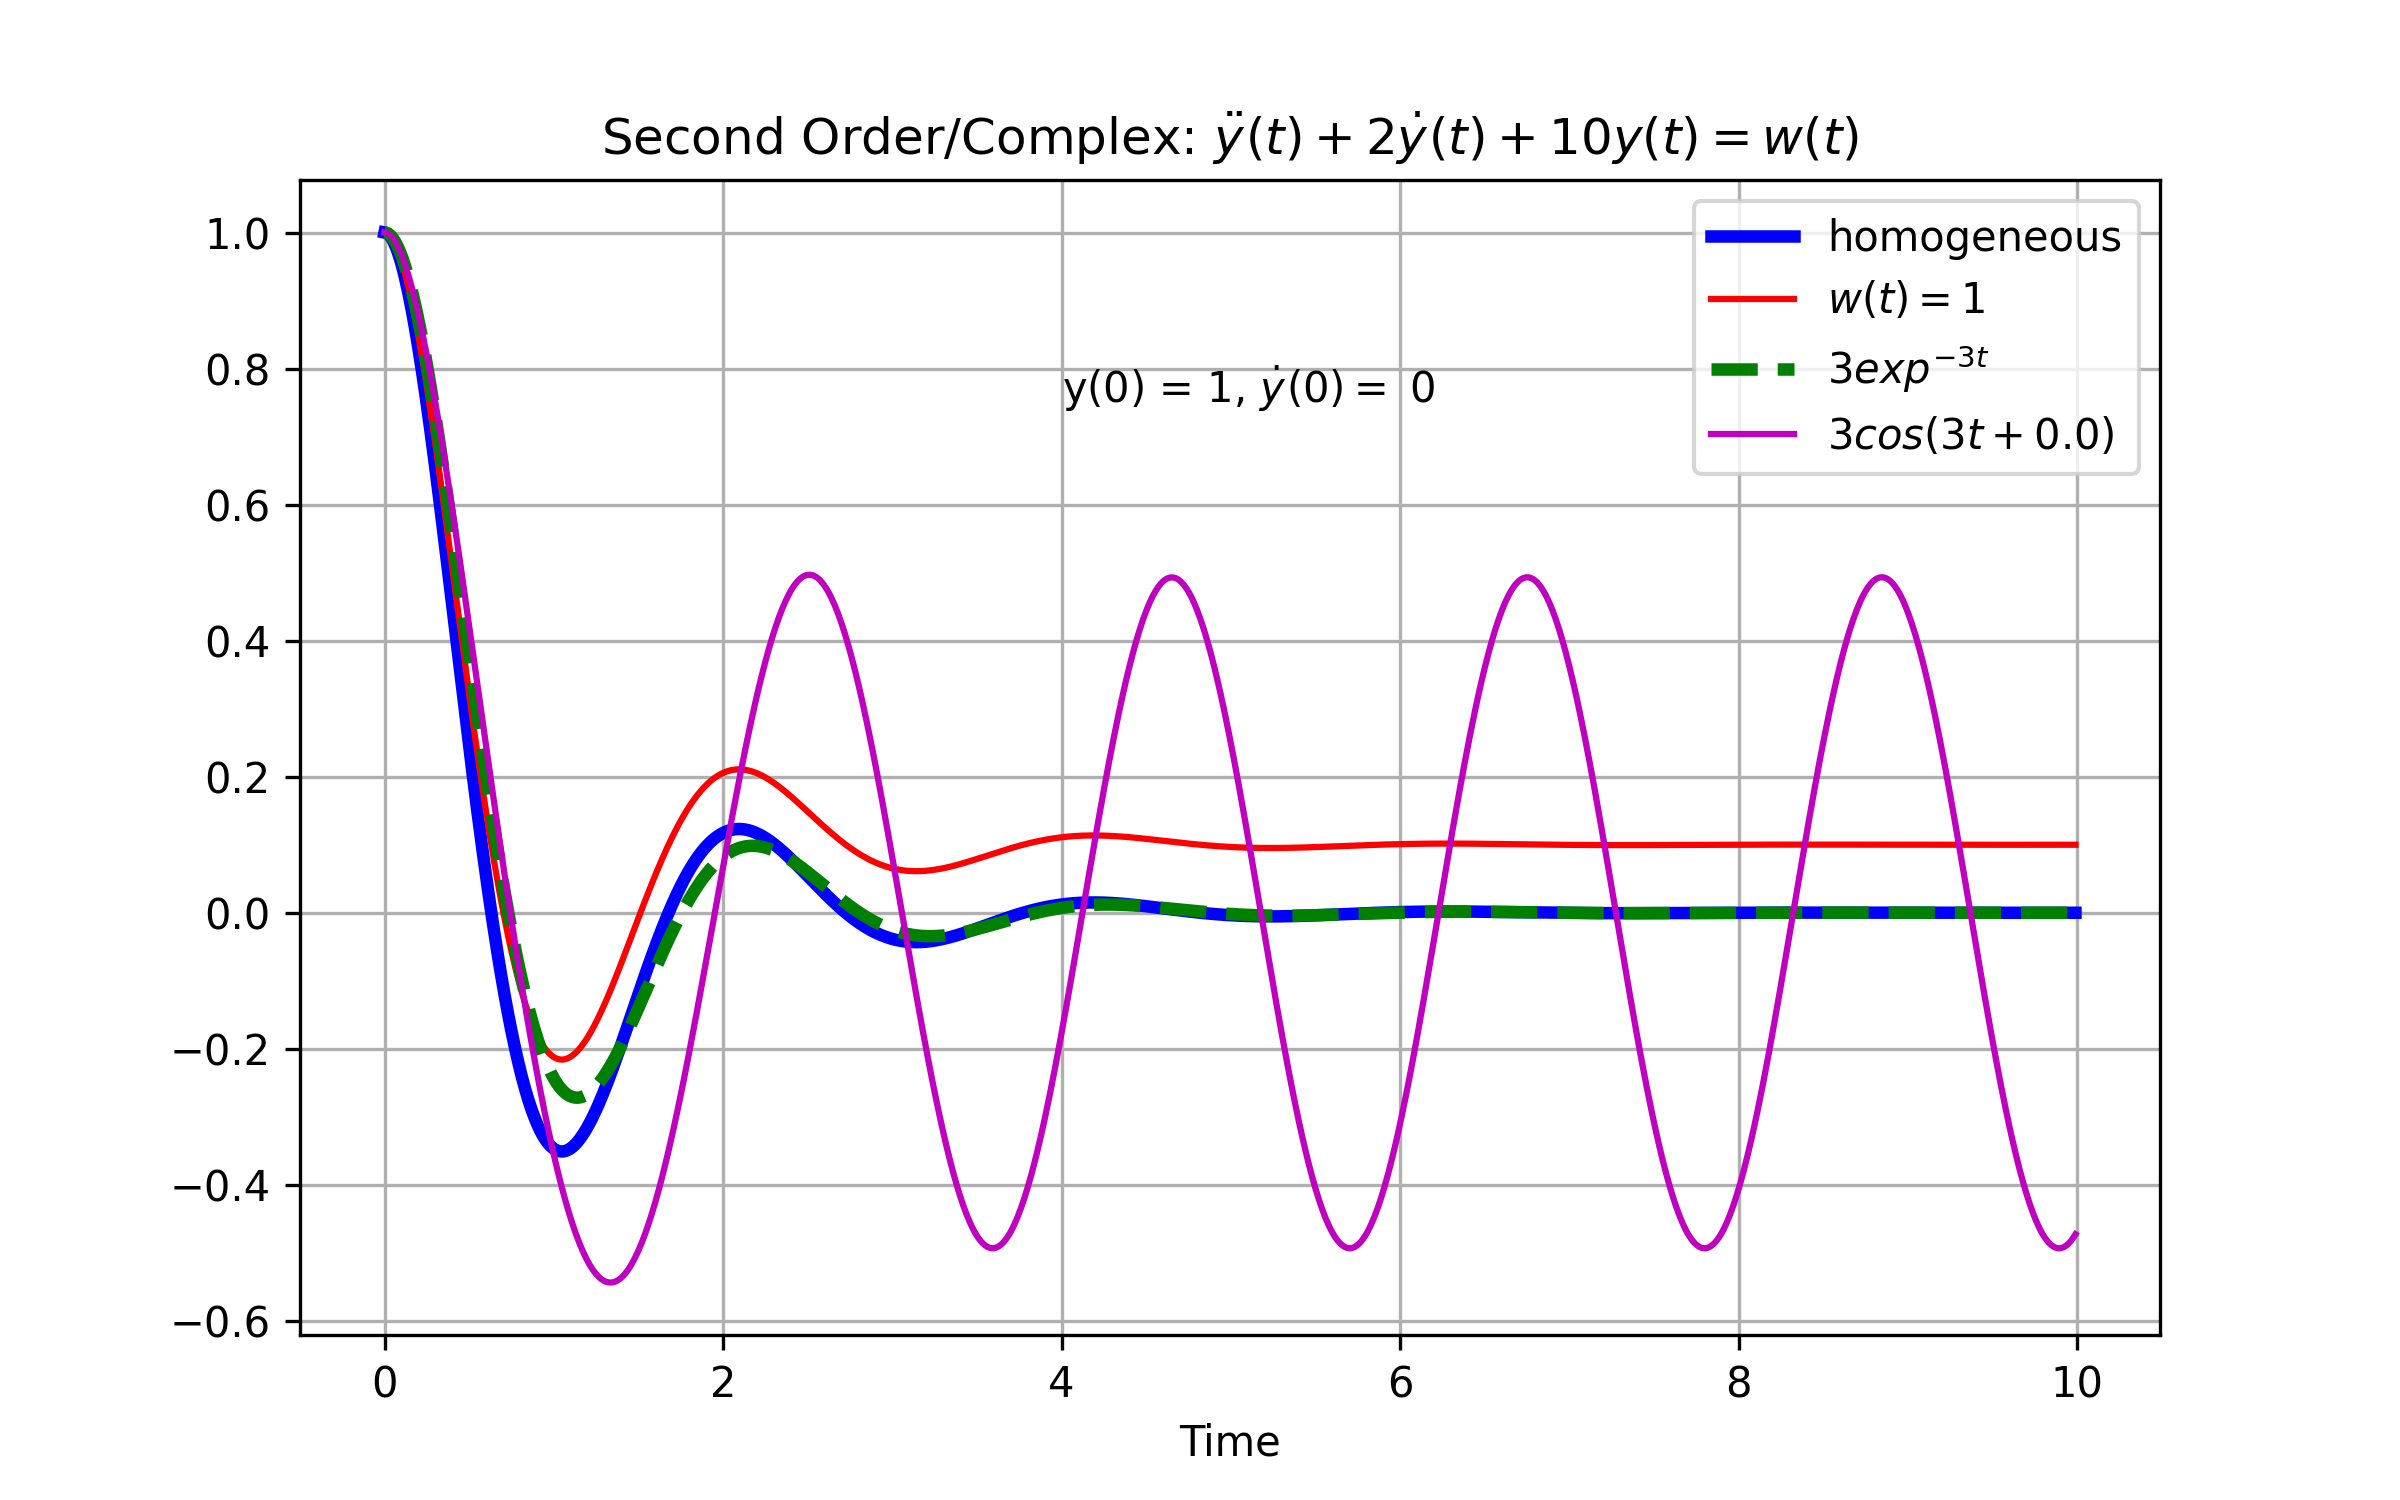
\includegraphics[width=6in]{figs/second_order_complex.png}
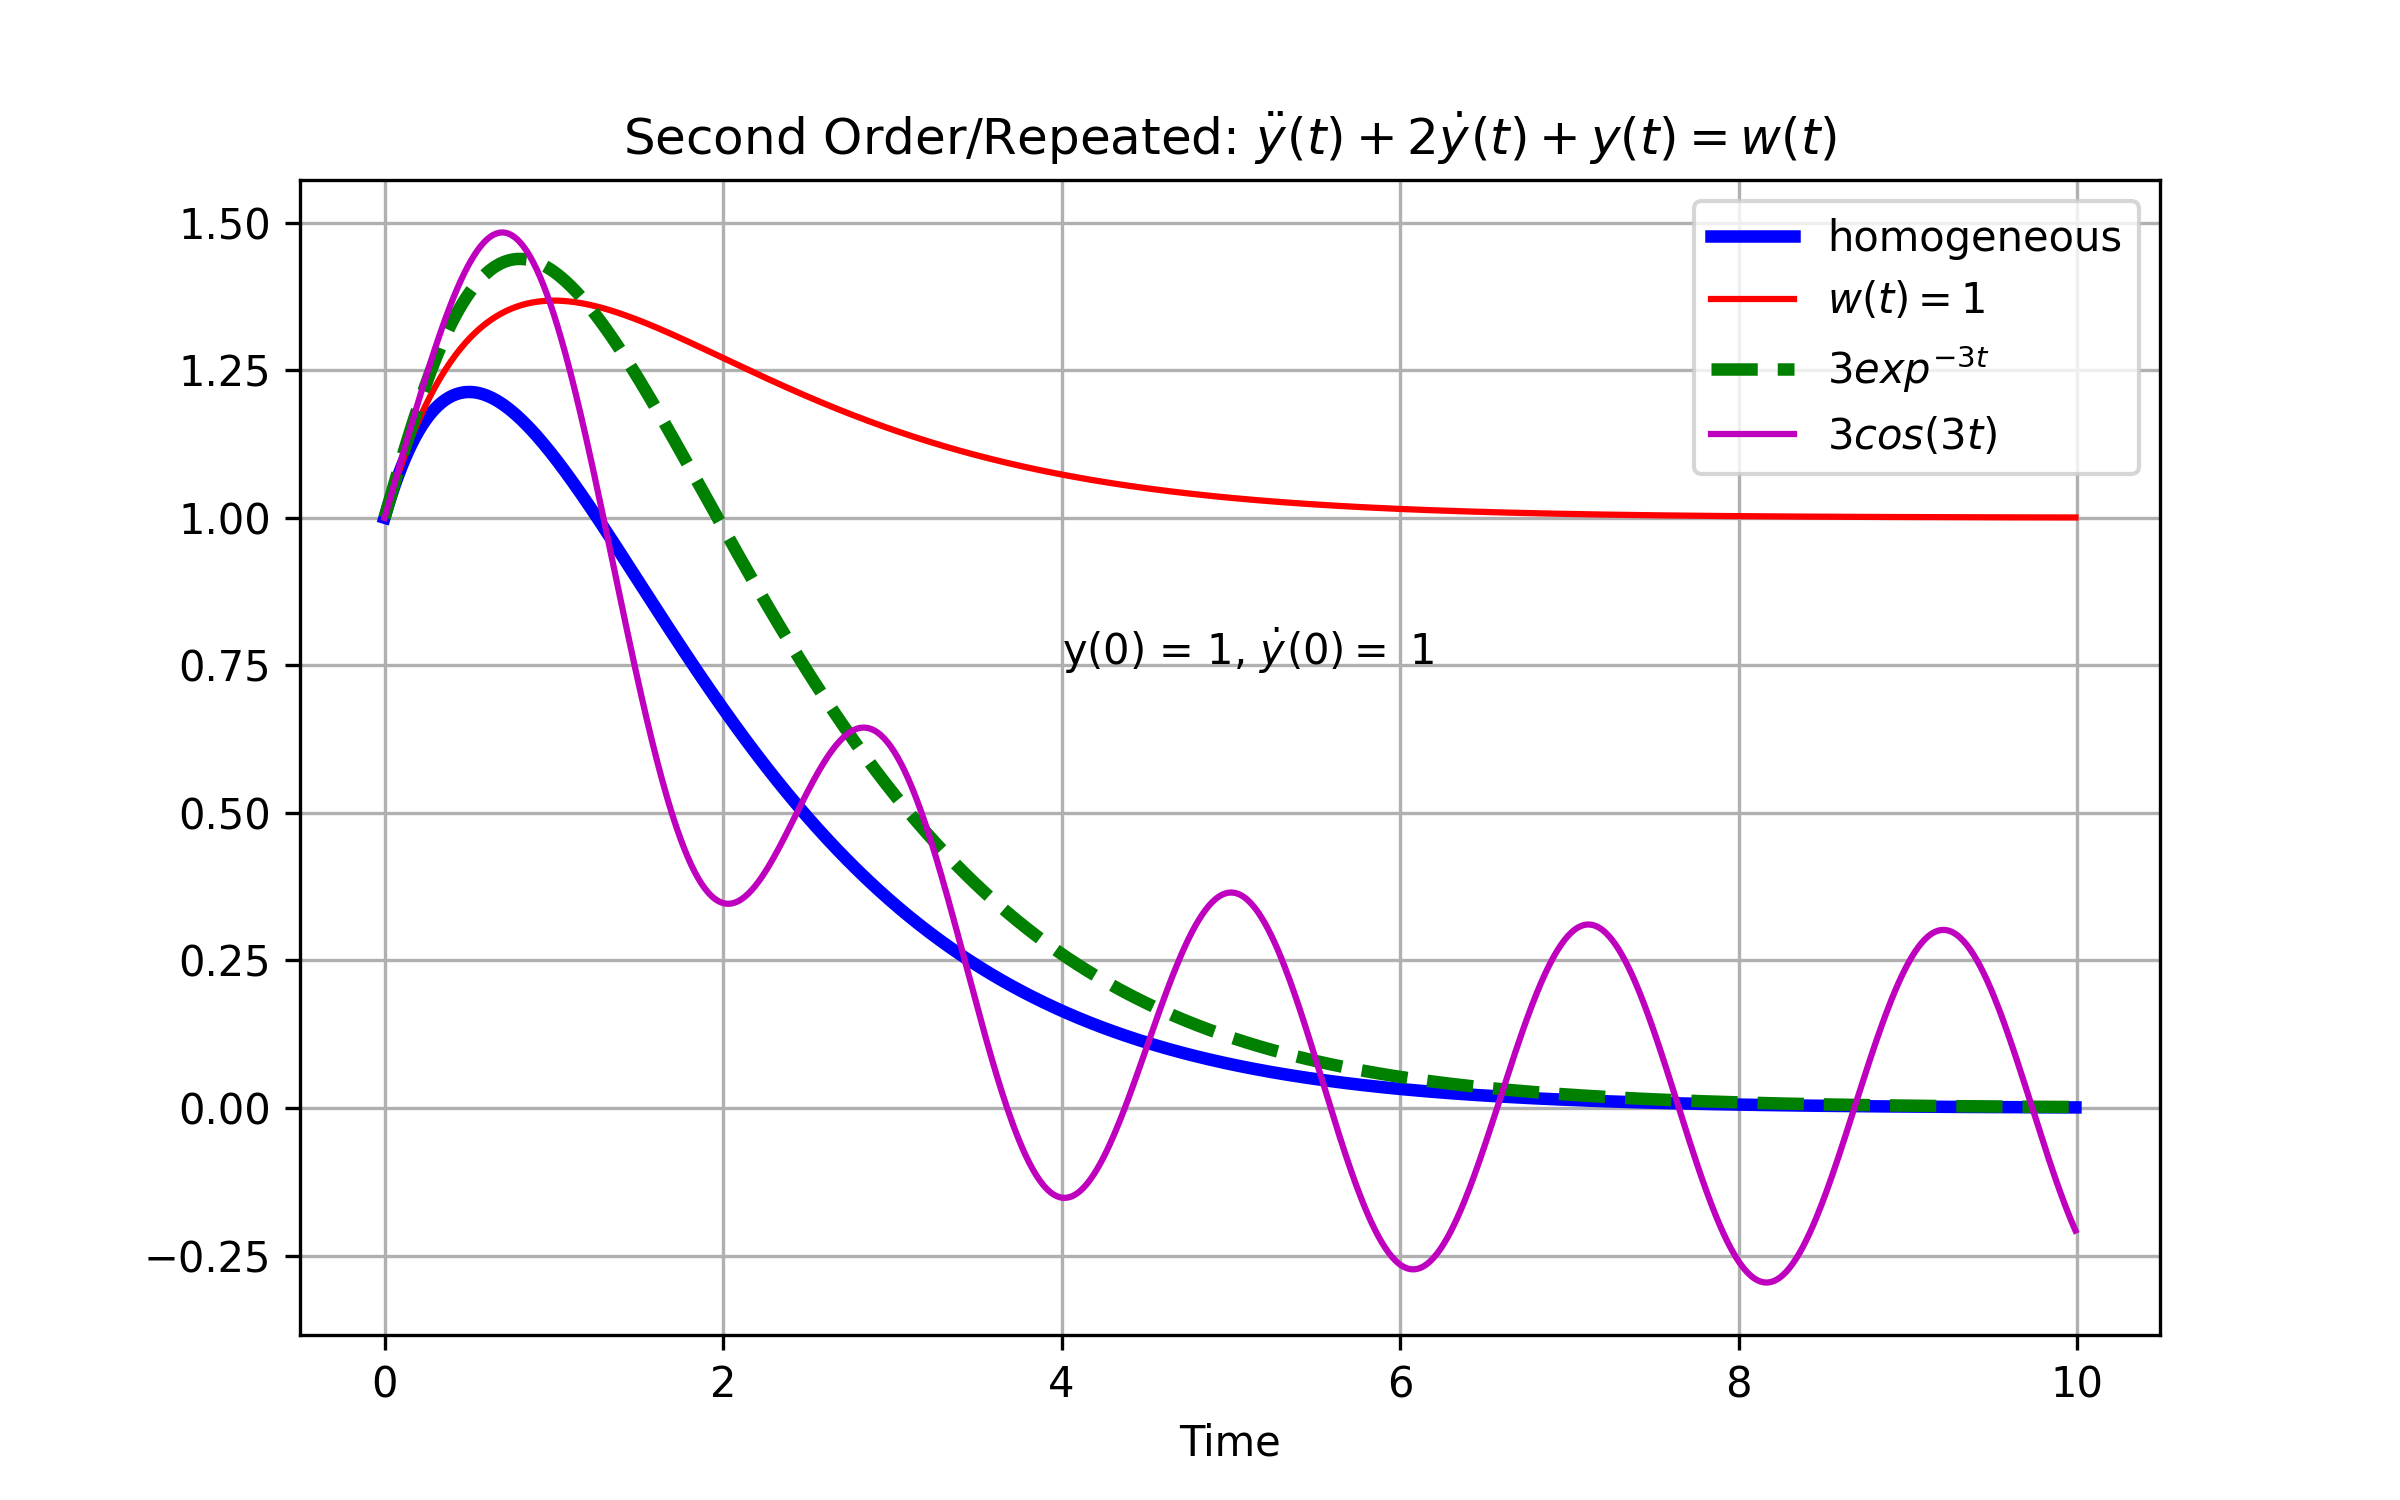
\includegraphics[width=6in]{figs/second_order_repeated.png}
\ec

\newpage
\noindent
\textbf{Numerically:} The numerical comparison script is also loaded directly.
\bc
\begin{center} \tiny
\textbf{\texttt{scripts/06\_numerical\_vs\_analytical.py}}
\lstinputlisting{scripts/06_numerical_vs_analytical.py}
\end{center}
\ec

\bc
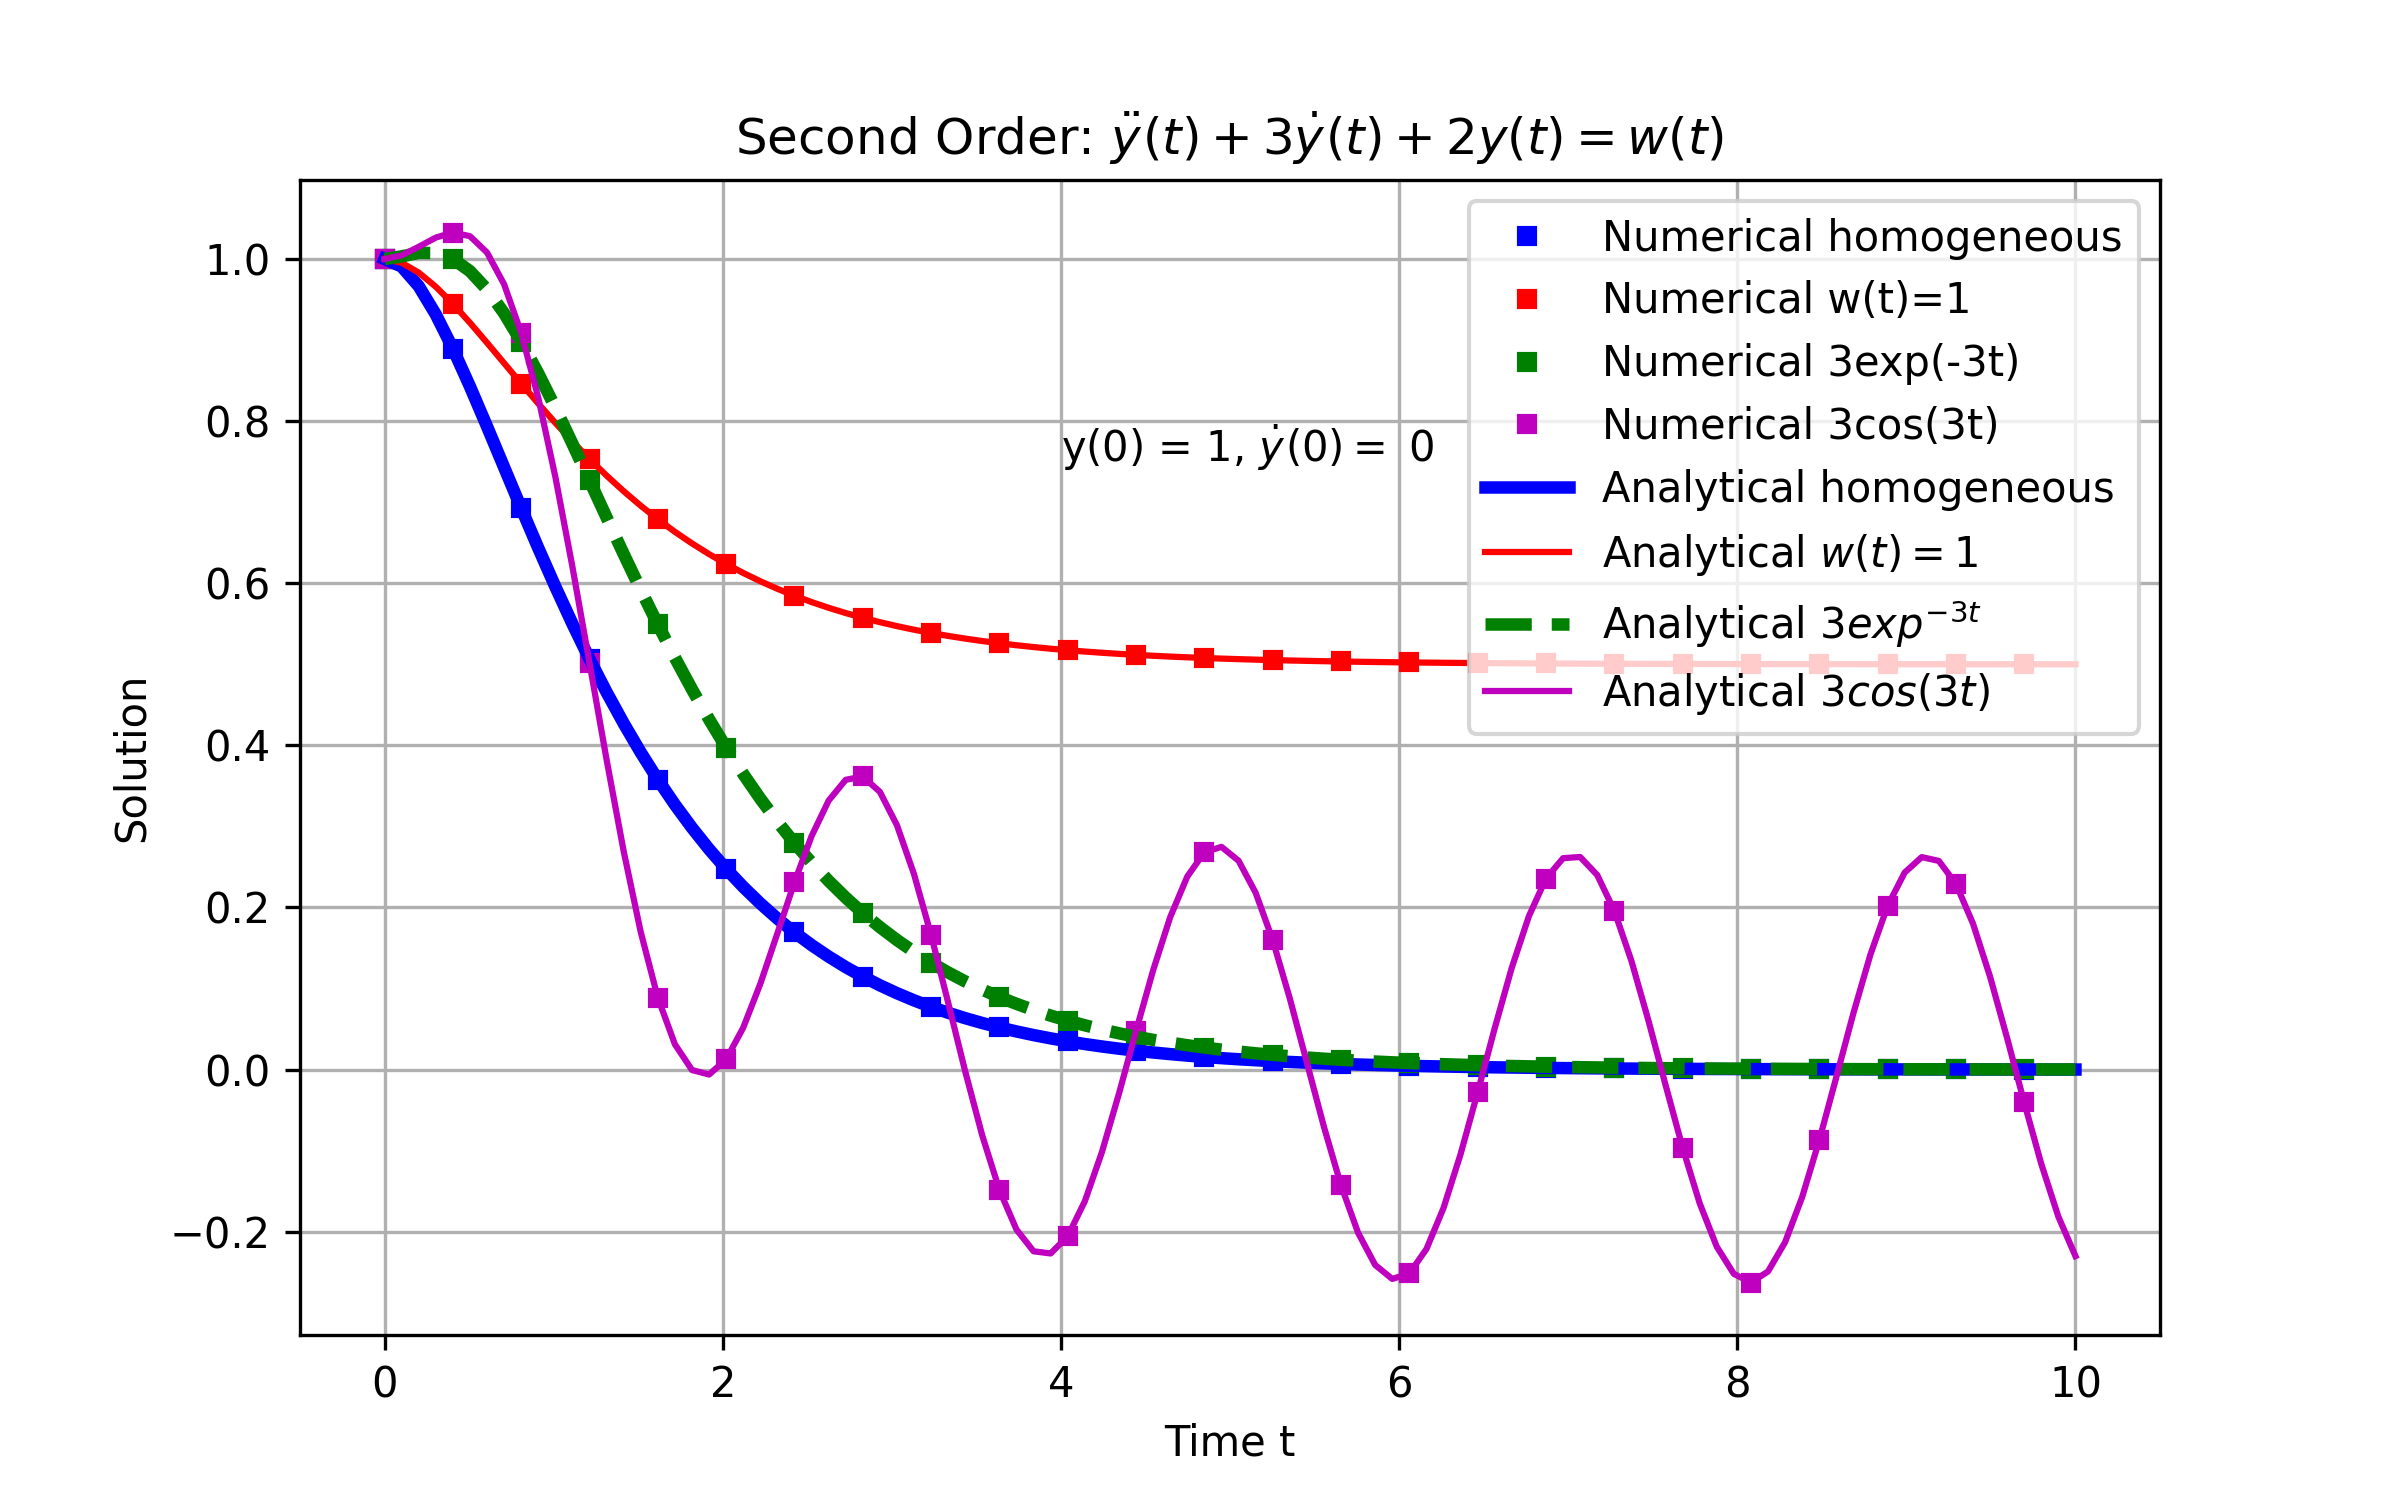
\includegraphics[width=6in]{figs/second_order_numerical_compare.png}
\ec
\end{document}